\section{Schematic}

The objective of this laboratory is to layout a two stage Miller OTA.

Figure \ref{fig:sch} shows the schematic of the OTA, including parameters for MOSFETs.

\begin{figure}[!htb]
	\centering
	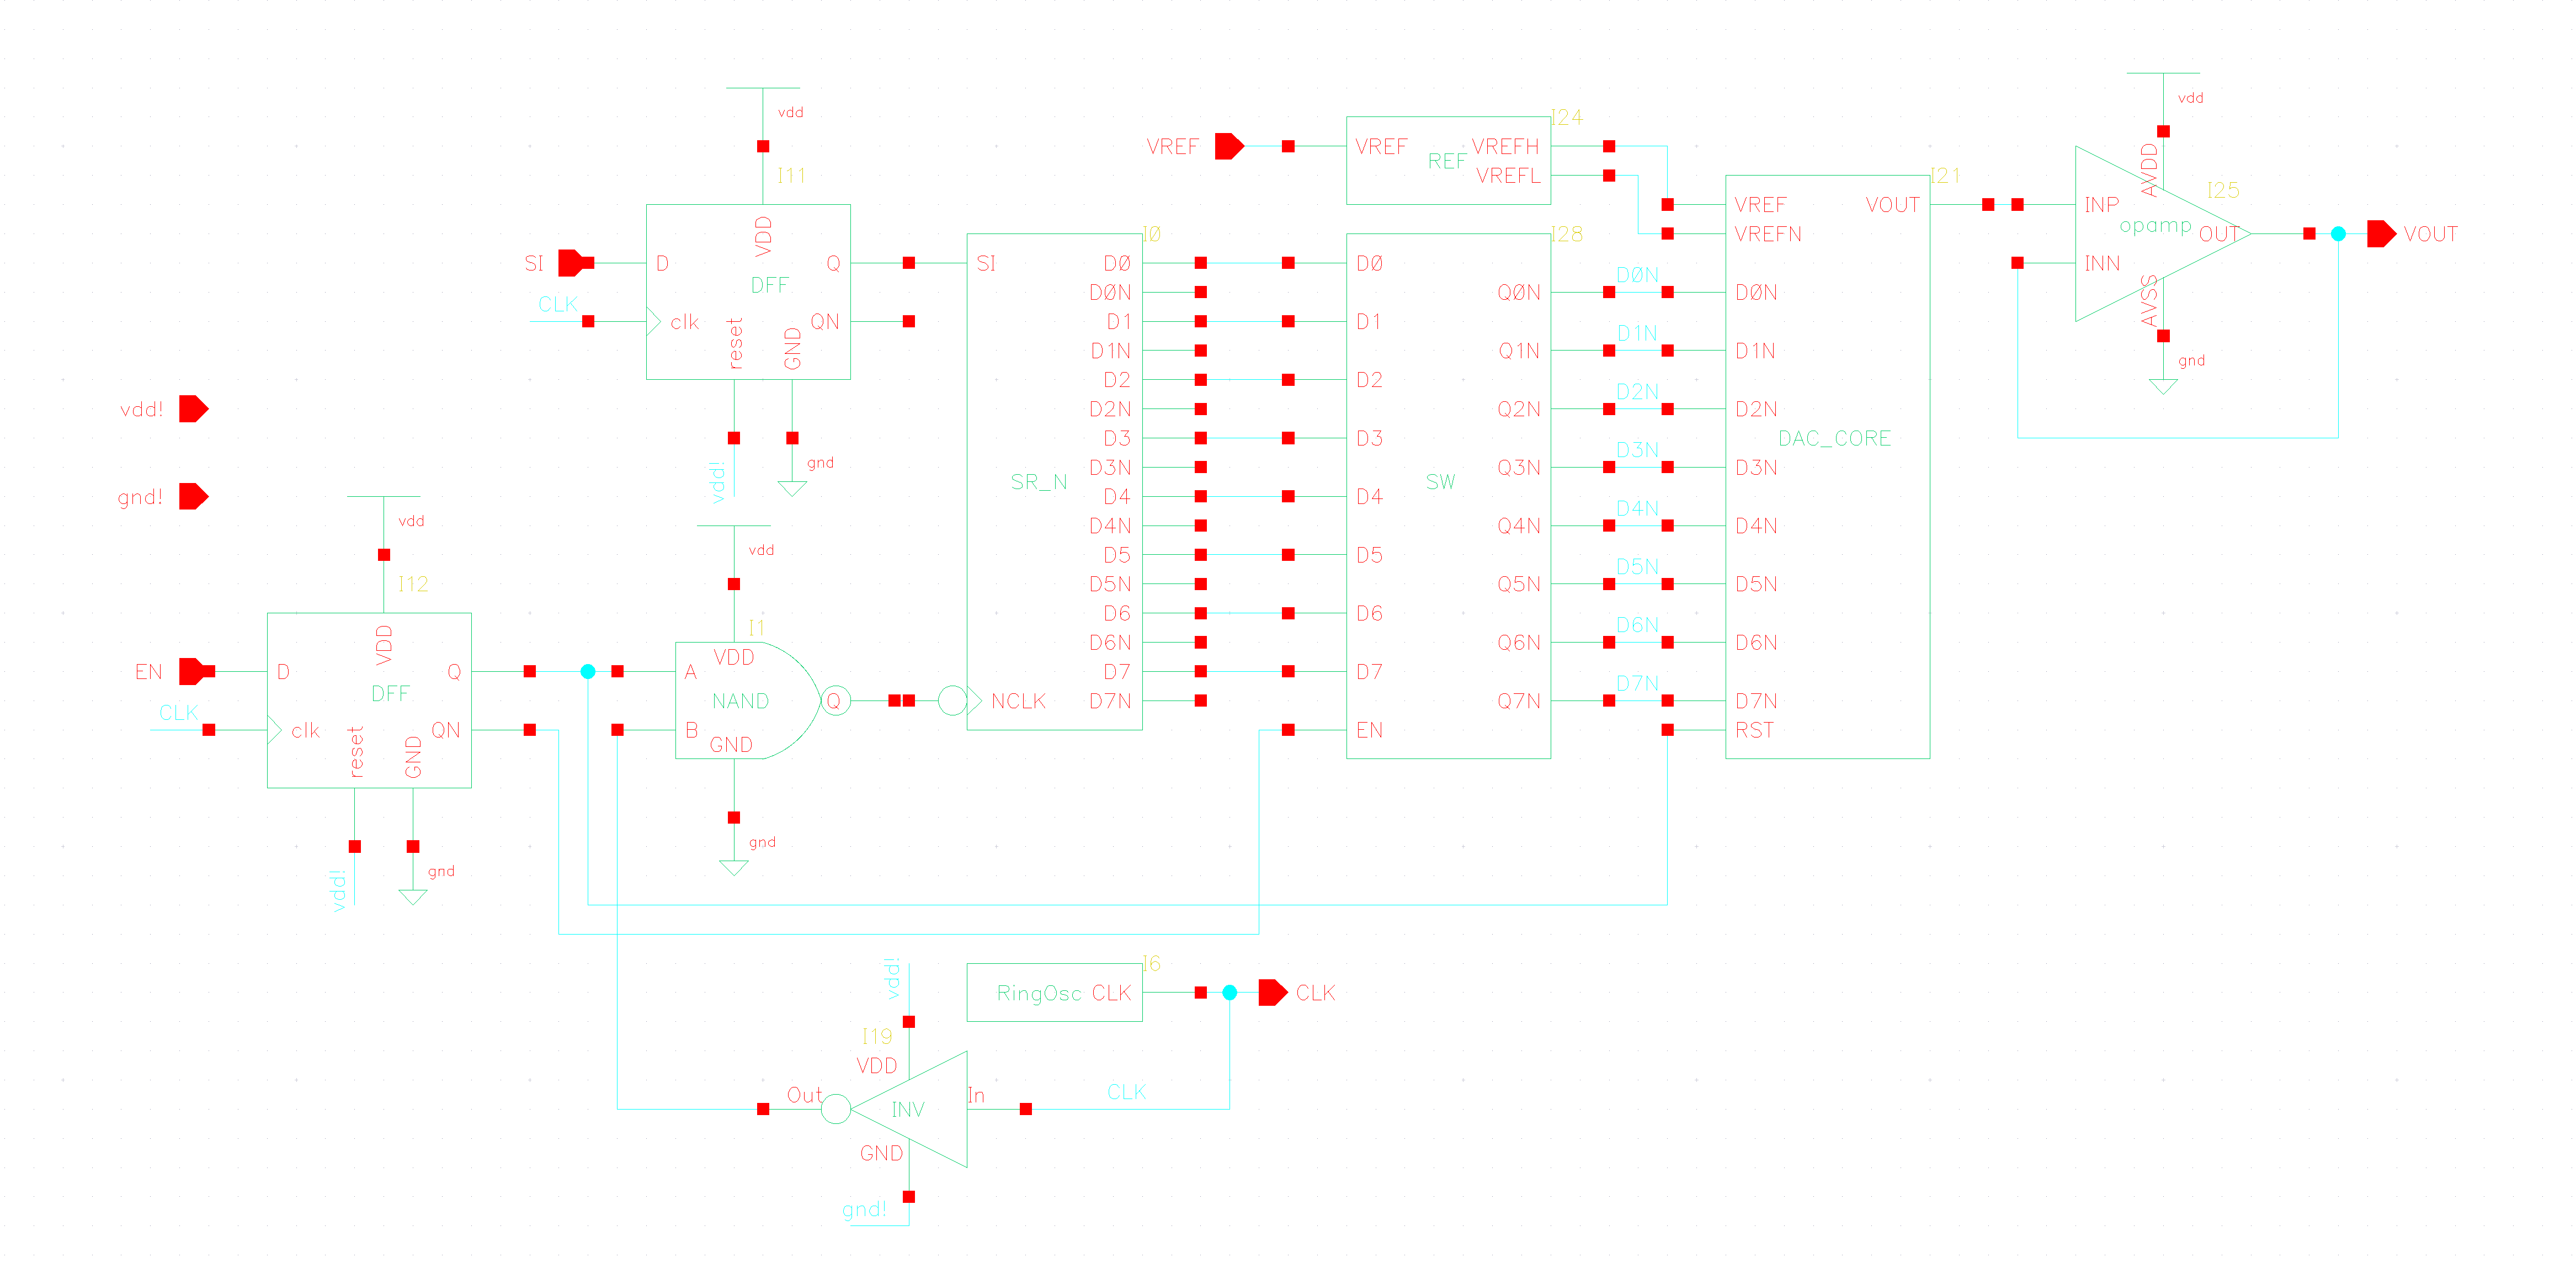
\includegraphics[width=\textwidth]{sch}
	\caption{Schematic including MOSFET parameters}
	\label{fig:sch}
\end{figure}

PM0 and PM1, the 2 PMOS transistors that forms the differential pair, were changed to a multiplication of 10 MOSFETs with channel width of $10 \mu m$ instead of $100 \mu m$ as in the notes, in order for better device matching between them using common centroid technique.

PM2 and PM4, the 2 PMOS transistors used in a current mirror configuration, were changed to use a base width of $6 \mu m$ with 4 and 16 fingers respectively. This is to match the other transistor PM5 used in the same current mirror configuration, which has a width of $6 \mu m$.

NM3, the common source NMOS amplifier, was changed to 8 fingers of width $4.75 \mu m$, to improve layout area efficiency. This also reduces gate resistance, compared with a MOSFET with very long gate width.
